\chapter{Discussing Fusion Power}

\label{chapter:power}

In a tokamak reactor, the main source of output power is fusion. Therefore, this chapter goes over a quick background of fusion power and describes a method for how to calculate the reactivity term that appears inside it. The particular method used for this reactivity approximation was done by Bosch and Hale in 1992.\cite{boschhale}

\section{Theoretical Background}

The natural place to start when introducing fusion energy is the binding energy per nucleon curve shown in \cref{fig:binding_energy}. As can be seen, this function reaches a maximum value around the element Iron (A=56). What this means at a basic level is: elements lighter than iron can \emph{fuse} into a heavier one (i.e.\ hydrogens into helium), whereas heavier elements can \emph{fission} into lighter ones (e.g.\ uranium into krypton and barium). This is what differentiates fission (uranium-fueled) reactors from fusion (hydrogen-fueled) ones. For fusion reactors, the most common reaction in a first-generation tokamak will be:
\begin{equation}
	{}^2H+ {}^3H \rightarrow {}^4 He + {}^1 n + E_F
\end{equation}
\myequations{Fusion Energy -- $E_F$}
\begin{equation}
	E_F = 17.6 \ \textnormal{MeV}
\end{equation}

\begin{figure}
	\centering
	\begin{adjustbox}{width=0.75\textwidth}
		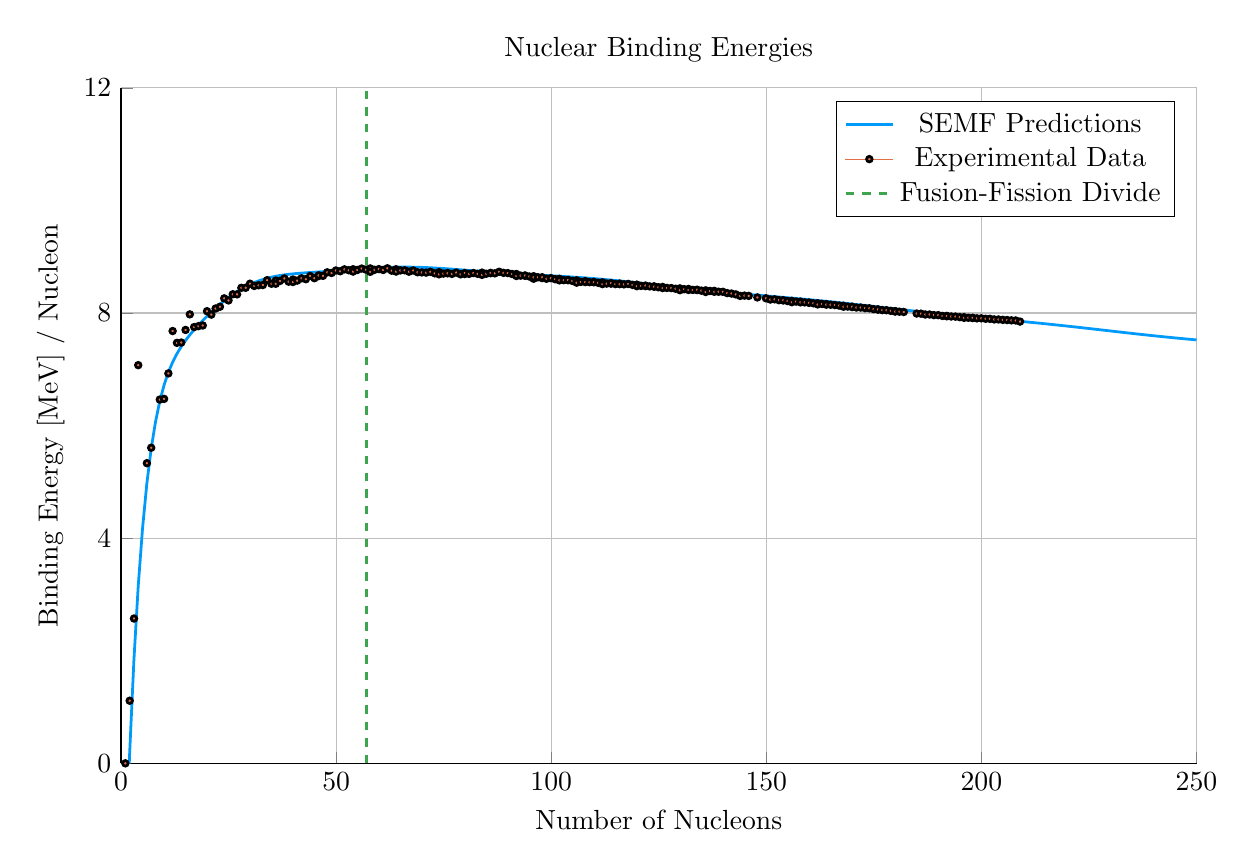
\begin{tikzpicture}[]
\begin{axis}[height = {101.6mm}, ylabel = {Binding Energy [MeV] / Nucleon}, title = {Nuclear Binding Energies}, xmin = {0}, xmax = {250}, ymax = {12}, xlabel = {Number of Nucleons}, {unbounded coords=jump, scaled x ticks = false, xticklabel style={rotate = 0}, xmajorgrids = true, xtick = {0.0,50.0,100.0,150.0,200.0,250.0}, xticklabels = {0,50,100,150,200,250}, xtick align = inside, axis lines* = left, scaled y ticks = false, yticklabel style={rotate = 0}, ymajorgrids = true, ytick = {0.0,4.0,8.0,12.0}, yticklabels = {0,4,8,12}, ytick align = inside, axis lines* = left,     xshift = 0.0mm,
    yshift = 0.0mm,
    axis background/.style={fill={rgb,1:red,1.00000000;green,1.00000000;blue,1.00000000}}
}, ymin = {0}, width = {152.4mm}]\addplot+ [color = {rgb,1:red,0.00000000;green,0.60560316;blue,0.97868012},
draw opacity=1.0,
line width=1,
solid,mark = none,
mark size = 2.0,
mark options = {
    color = {rgb,1:red,0.00000000;green,0.00000000;blue,0.00000000}, draw opacity = 1.0,
    fill = {rgb,1:red,0.00000000;green,0.60560316;blue,0.97868012}, fill opacity = 1.0,
    line width = 1,
    rotate = 0,
    solid
}]coordinates {
(0.0, -4.60355222317376)
(1.0, -1.9423714030316184)
(2.0, 0.17174117296689762)
(3.0, 1.84096399661781)
(4.0, 3.151140198415331)
(5.0, 4.173923283645508)
(6.0, 4.968707102167827)
(7.0, 5.58435286219236)
(8.0, 6.060726579422419)
(9.0, 6.430060629330575)
(10.0, 6.718153095546762)
(11.0, 6.9454184281365565)
(12.0, 7.127802582683796)
(13.0, 7.277575339898747)
(14.0, 7.404011936438574)
(15.0, 7.513975496904414)
(16.0, 7.6124110668622125)
(17.0, 7.702761326082542)
(18.0, 7.78731332582606)
(19.0, 7.867484857048368)
(20.0, 7.94405832862659)
(21.0, 8.017369324812918)
(22.0, 8.087456325980316)
(23.0, 8.154177421651507)
(24.0, 8.217299223743723)
(25.0, 8.276562603700583)
(26.0, 8.331729331502007)
(27.0, 8.382613188387339)
(28.0, 8.429098658726296)
(29.0, 8.471149879476823)
(30.0, 8.508812137244952)
(31.0, 8.542207851888847)
(32.0, 8.571528670372789)
(33.0, 8.59702501341144)
(34.0, 8.618994168442093)
(35.0, 8.637767803574754)
(36.0, 8.653699586296018)
(37.0, 8.66715342570664)
(38.0, 8.678492715810727)
(39.0, 8.688070837773061)
(40.0, 8.696223079017631)
(41.0, 8.703260044649955)
(42.0, 8.709462569971606)
(43.0, 8.715078090099894)
(44.0, 8.720318382160027)
(45.0, 8.725358565619327)
(46.0, 8.730337225625941)
(47.0, 8.735357511312394)
(48.0, 8.74048905473126)
(49.0, 8.745770555203375)
(50.0, 8.75121287745749)
(51.0, 8.756802519009028)
(52.0, 8.762505312039806)
(53.0, 8.76827023680805)
(54.0, 8.774033236747258)
(55.0, 8.779720939428142)
(56.0, 8.785254201806225)
(57.0, 8.790551412530785)
(58.0, 8.795531497975329)
(59.0, 8.800116592037245)
(60.0, 8.804234342184401)
(61.0, 8.80781983582066)
(62.0, 8.810817141406119)
(63.0, 8.813180468193043)
(64.0, 8.814874956307978)
(65.0, 8.815877115972366)
(66.0, 8.816174940266126)
(67.0, 8.815767720260371)
(68.0, 8.814665595039155)
(69.0, 8.81288887100591)
(70.0, 8.810467147004726)
(71.0, 8.807438281492448)
(72.0, 8.803847238531759)
(73.0, 8.799744847854736)
(74.0, 8.795186513048279)
(75.0, 8.790230899697235)
(76.0, 8.78493863297573)
(77.0, 8.77937103143497)
(78.0, 8.773588900376659)
(79.0, 8.767651405642294)
(80.0, 8.76161504469066)
(81.0, 8.755532729350353)
(82.0, 8.749452990095264)
(83.0, 8.743419310368836)
(84.0, 8.737469594886402)
(85.0, 8.731635772840807)
(86.0, 8.725943537136203)
(87.0, 8.72041221331207)
(88.0, 8.71505475533288)
(89.0, 8.709877858732526)
(90.0, 8.704882183589692)
(91.0, 8.700062675015097)
(92.0, 8.695408972428076)
(93.0, 8.690905892370129)
(94.0, 8.686533974543913)
(95.0, 8.682270076666686)
(96.0, 8.678088004492896)
(97.0, 8.67395916751817)
(98.0, 8.669853242580963)
(99.0, 8.665738837927783)
(100.0, 8.661584144823571)
(101.0, 8.657357563363785)
(102.0, 8.65302830389561)
(103.0, 8.648566937275728)
(104.0, 8.643945904303443)
(105.0, 8.639139972215713)
(106.0, 8.634126623930722)
(107.0, 8.628886396202454)
(108.0, 8.623403143699367)
(109.0, 8.617664241985338)
(110.0, 8.611660722384958)
(111.0, 8.605387333426602)
(112.0, 8.598842559648038)
(113.0, 8.592028549789976)
(114.0, 8.58495101272171)
(115.0, 8.57761904583371)
(116.0, 8.570044915671591)
(117.0, 8.562243798972087)
(118.0, 8.554233483777885)
(119.0, 8.546034047126547)
(120.0, 8.537667484888594)
(121.0, 8.52915735205801)
(122.0, 8.520528366411522)
(123.0, 8.511806023276883)
(124.0, 8.503016188183416)
(125.0, 8.494184739476726)
(126.0, 8.48533715574106)
(127.0, 8.476498181446992)
(128.0, 8.467691475241981)
(129.0, 8.458939312854039)
(130.0, 8.450262302915618)
(131.0, 8.441679114253642)
(132.0, 8.433206278428624)
(133.0, 8.424858004233645)
(134.0, 8.416646056664081)
(135.0, 8.408579640871974)
(136.0, 8.40066533194409)
(137.0, 8.392907065338754)
(138.0, 8.38530615381601)
(139.0, 8.377861360242079)
(140.0, 8.370568923080928)
(141.0, 8.363422766320568)
(142.0, 8.356414619878997)
(143.0, 8.349534089567673)
(144.0, 8.34276906318144)
(145.0, 8.336105786797518)
(146.0, 8.329529164601073)
(147.0, 8.323022920758717)
(148.0, 8.316570078748192)
(149.0, 8.310152950625312)
(150.0, 8.303753629008376)
(151.0, 8.297354097141259)
(152.0, 8.290936673163188)
(153.0, 8.284484104508877)
(154.0, 8.277979817957576)
(155.0, 8.271408214247263)
(156.0, 8.26475482066996)
(157.0, 8.258006702964753)
(158.0, 8.251151969185319)
(159.0, 8.244180856070077)
(160.0, 8.237085161410096)
(161.0, 8.229858338085972)
(162.0, 8.222496057535484)
(163.0, 8.214995696045428)
(164.0, 8.207356657383283)
(165.0, 8.199580440708676)
(166.0, 8.191669837642781)
(167.0, 8.183630071172871)
(168.0, 8.175467743710037)
(169.0, 8.167191164794605)
(170.0, 8.158809617848195)
(171.0, 8.150334504183075)
(172.0, 8.14177744744961)
(173.0, 8.133151658440163)
(174.0, 8.124470878350785)
(175.0, 8.115749356192289)
(176.0, 8.107001644999418)
(177.0, 8.098242201855552)
(178.0, 8.089486091809402)
(179.0, 8.080747293619883)
(180.0, 8.072039470032013)
(181.0, 8.063376210895715)
(182.0, 8.054769614767046)
(183.0, 8.0462311233693)
(184.0, 8.037770796191257)
(185.0, 8.029398175968147)
(186.0, 8.021119837562082)
(187.0, 8.012942869232848)
(188.0, 8.004870739363358)
(189.0, 7.996906945184318)
(190.0, 7.9890525617077115)
(191.0, 7.981307878966942)
(192.0, 7.973670320833624)
(193.0, 7.966137802437683)
(194.0, 7.9587038074885585)
(195.0, 7.951361389542597)
(196.0, 7.94410538135961)
(197.0, 7.936926816592529)
(198.0, 7.929813814345658)
(199.0, 7.9227553501678285)
(200.0, 7.9157413728397765)
(201.0, 7.908760790229455)
(202.0, 7.901797768231368)
(203.0, 7.894842094438137)
(204.0, 7.887880452358307)
(205.0, 7.880899530438714)
(206.0, 7.873885760576088)
(207.0, 7.866828874177291)
(208.0, 7.859716917643159)
(209.0, 7.8525395883864215)
(210.0, 7.845285908240645)
(211.0, 7.837951508078004)
(212.0, 7.830524697560121)
(213.0, 7.823000336600177)
(214.0, 7.815372950142774)
(215.0, 7.807640337638273)
(216.0, 7.799801848697318)
(217.0, 7.791862143087951)
(218.0, 7.783807545643804)
(219.0, 7.77565377827491)
(220.0, 7.767399807770702)
(221.0, 7.759051137290531)
(222.0, 7.750623260339327)
(223.0, 7.742107372543793)
(224.0, 7.73352368610323)
(225.0, 7.724889447747704)
(226.0, 7.7162018331861555)
(227.0, 7.707489994804505)
(228.0, 7.698747655296494)
(229.0, 7.689999393671084)
(230.0, 7.6812378105210035)
(231.0, 7.672517835584716)
(232.0, 7.663814423654281)
(233.0, 7.655151966005575)
(234.0, 7.646557126836435)
(235.0, 7.638013924639547)
(236.0, 7.629551857020474)
(237.0, 7.62119791263829)
(238.0, 7.612907202266693)
(239.0, 7.604745643355369)
(240.0, 7.596673359765863)
(241.0, 7.588747960772381)
(242.0, 7.580936729929124)
(243.0, 7.573223292898663)
(244.0, 7.565631417500911)
(245.0, 7.5581978936317435)
(246.0, 7.550821503884376)
(247.0, 7.543623555302642)
(248.0, 7.536478832551908)
(249.0, 7.529431955026017)
(250.0, 7.522541556397873)
};
\addlegendentry{SEMF Predictions}
\addplot+[draw=none, color = {rgb,1:red,0.88887350;green,0.43564919;blue,0.27812294},
draw opacity=1.0,
line width=0,
solid,mark = *,
mark size = 1.0,
mark options = {
    color = {rgb,1:red,0.00000000;green,0.00000000;blue,0.00000000}, draw opacity = 1.0,
    fill = {rgb,1:red,0.88887350;green,0.43564919;blue,0.27812294}, fill opacity = 1.0,
    line width = 1,
    rotate = 0,
    solid
}] coordinates {
(1.007825, 0.0)
(2.0141018, 1.1122865)
(3.0160293, 2.572686)
(4.0026032, 7.07391825)
(6.0151223, 5.332427333)
(7.016004, 5.606360857)
(9.0121821, 6.462767333)
(10.012937, 6.4750702)
(11.0093055, 6.927709364)
(12.0, 7.680145917)
(13.0033548, 7.469851)
(14.003074, 7.475616429)
(15.0001089, 7.699461867)
(15.9949146, 7.976208688)
(16.9991315, 7.750745)
(17.9991604, 7.7670585)
(18.9984032, 7.779019)
(19.9924402, 8.0322426)
(20.9938467, 7.971712381)
(21.9913855, 8.080450591)
(22.9897697, 8.111479391)
(23.9850419, 8.260703417)
(24.985837, 8.2235022)
(25.982593, 8.333870538)
(26.9815384, 8.331553704)
(27.9769265, 8.447745714)
(28.9764947, 8.448635759)
(29.9737702, 8.5206538)
(30.9737615, 8.481183452)
(31.9720707, 8.493145938)
(32.9714585, 8.497643667)
(33.9678668, 8.583505059)
(34.9688527, 8.520280229)
(35.9670809, 8.575386889)
(35.9675463, 8.5198805)
(36.9659026, 8.570282811)
(37.9627322, 8.614281105)
(38.9637069, 8.557018564)
(39.9623831, 8.595261375)
(39.9625912, 8.551298525)
(40.961826, 8.576058732)
(41.9586183, 8.616553905)
(42.9587668, 8.600656907)
(43.9554811, 8.658187182)
(44.9559102, 8.618876822)
(45.9526295, 8.656400587)
(45.9536928, 8.668884283)
(46.9517638, 8.661109447)
(47.9479471, 8.722890208)
(48.9478708, 8.711042755)
(49.9447921, 8.75560424)
(50.9439637, 8.741976863)
(51.9405119, 8.775867173)
(52.9406538, 8.760080585)
(53.9388849, 8.777838241)
(53.9396148, 8.736271611)
(54.9380496, 8.764914764)
(55.9349421, 8.790248321)
(56.9353987, 8.770174263)
(57.9332805, 8.792144241)
(57.9353479, 8.731962534)
(58.9332002, 8.767933983)
(59.9307906, 8.78069255)
(60.9310604, 8.764943607)
(61.9283488, 8.794496597)
(62.9296011, 8.752082952)
(63.9279696, 8.777416234)
(63.9291466, 8.735836984)
(64.9277937, 8.757037815)
(65.9260368, 8.759590848)
(66.9271309, 8.734107179)
(67.9248476, 8.755637676)
(68.9255809, 8.724482)
(69.9242504, 8.721679686)
(70.924705, 8.717574859)
(71.9220762, 8.731742861)
(72.9234594, 8.705046356)
(73.9211782, 8.725197459)
(73.9224766, 8.6877095)
(74.9215964, 8.70085368)
(75.9192141, 8.711474776)
(75.9214027, 8.705237934)
(76.9199146, 8.694687091)
(77.9173095, 8.717805526)
(78.9183376, 8.68759657)
(79.916378, 8.6929306)
(79.9165218, 8.710815425)
(80.9162911, 8.695915321)
(81.9134846, 8.71063828)
(82.914136, 8.695625024)
(83.9115066, 8.717350548)
(83.9134248, 8.677451726)
(84.9117893, 8.697447294)
(85.9092624, 8.708440733)
(85.9106103, 8.712034709)
(86.9088793, 8.705218437)
(87.9056143, 8.732575159)
(88.9058479, 8.713910393)
(89.9047037, 8.709920922)
(90.905645, 8.693268154)
(91.9050401, 8.692631598)
(91.9068105, 8.657698924)
(92.9063775, 8.66414257)
(93.9050876, 8.662296372)
(93.9063158, 8.666771426)
(94.9058415, 8.648682926)
(95.9046789, 8.65394974)
(95.9075977, 8.609329219)
(95.9082757, 8.635348635)
(96.906021, 8.635054443)
(97.9052871, 8.620312122)
(97.9054078, 8.635130592)
(98.9059393, 8.608630253)
(99.9042197, 8.61927551)
(100.9055822, 8.601283307)
(101.9043495, 8.607345284)
(101.9056077, 8.580514941)
(102.9055042, 8.584102893)
(103.9040349, 8.584809519)
(103.9054301, 8.587358327)
(104.905084, 8.570611867)
(105.9034831, 8.579970453)
(105.906458, 8.539066528)
(106.905093, 8.553889477)
(107.9038945, 8.567003037)
(107.9041834, 8.550022833)
(108.9047555, 8.547919321)
(109.9030056, 8.551293391)
(109.9051524, 8.547338309)
(110.9041816, 8.537100027)
(111.9027572, 8.544787813)
(111.9048208, 8.513654438)
(112.9040612, 8.522924912)
(113.9027818, 8.522555167)
(113.9033581, 8.531571772)
(114.903346, 8.514061435)
(115.9017441, 8.523107595)
(115.9047554, 8.512415397)
(116.9029538, 8.509615906)
(117.9016063, 8.516538458)
(118.9033089, 8.499470176)
(119.9021966, 8.504536442)
(119.9040199, 8.47734375)
(120.903818, 8.48200724)
(121.9030471, 8.478115393)
(121.9034401, 8.487940057)
(122.9042157, 8.472318821)
(123.9028195, 8.473263645)
(123.9052746, 8.467438726)
(124.9044247, 8.458085936)
(125.9033055, 8.463290746)
(125.9042689, 8.443750778)
(126.9044684, 8.445514346)
(127.9035304, 8.443305016)
(128.9047795, 8.431402163)
(129.9035079, 8.437744138)
(129.9063105, 8.4056265)
(130.9050819, 8.423754511)
(131.9041545, 8.427628947)
(131.9050562, 8.409412727)
(132.9054469, 8.41001582)
(133.9045033, 8.40820859)
(133.9053945, 8.413690821)
(134.9056827, 8.39757577)
(135.9045701, 8.402797926)
(135.9071436, 8.373666206)
(136.9058214, 8.391869759)
(137.9052413, 8.39346358)
(137.9059856, 8.377100848)
(138.9063482, 8.37809918)
(139.905434, 8.376402064)
(140.9076477, 8.354065376)
(141.9077186, 8.346099423)
(142.9098096, 8.330557867)
(143.9119947, 8.303756715)
(144.9125688, 8.309256297)
(145.9131121, 8.30416076)
(147.9168885, 8.277245601)
(149.9172715, 8.26169108)
(150.919846, 8.239366947)
(151.9197282, 8.244130184)
(152.9212262, 8.228767745)
(153.9208623, 8.224866201)
(153.9222053, 8.226903344)
(154.9226188, 8.213319839)
(155.9221196, 8.215390718)
(155.9242783, 8.192470455)
(156.9239567, 8.203572854)
(157.9241005, 8.20188807)
(157.9244046, 8.190191728)
(158.9253431, 8.188866572)
(159.9251937, 8.184111788)
(159.9270506, 8.183081056)
(160.9269296, 8.173367894)
(161.9267947, 8.173513907)
(161.9287749, 8.152468833)
(162.9287275, 8.16184127)
(163.9291712, 8.158769561)
(163.929197, 8.149082091)
(164.9303192, 8.147017042)
(165.93029, 8.142011898)
(166.9320454, 8.131797198)
(167.9323678, 8.129650298)
(167.9338945, 8.111871631)
(168.9342111, 8.114515675)
(169.9347587, 8.106659294)
(169.9354603, 8.112018182)
(170.9363223, 8.097934655)
(171.9363777, 8.097480244)
(172.9382068, 8.087480665)
(173.9388581, 8.083900891)
(174.9407679, 8.069192943)
(175.9414018, 8.061404835)
(175.9425684, 8.064120898)
(176.94322, 8.051892299)
(177.9436977, 8.049501567)
(178.9458151, 8.038604905)
(179.9465488, 8.0349901)
(179.9467057, 8.025484889)
(180.9479963, 8.023418619)
(181.9482055, 8.01831256)
(184.9529557, 7.991024865)
(185.9543622, 7.988619242)
(186.9557479, 7.973791439)
(187.955836, 7.973874356)
(188.9581449, 7.963010111)
(189.9584452, 7.962108089)
(190.9605912, 7.94811756)
(191.9610352, 7.942530948)
(191.961479, 7.948527021)
(192.9629237, 7.938136917)
(193.9626636, 7.936039562)
(194.9647744, 7.926650138)
(195.9649349, 7.926625776)
(195.9658148, 7.914460474)
(196.9665516, 7.915744218)
(197.9667518, 7.911637121)
(197.967876, 7.914250535)
(198.9682625, 7.905367905)
(199.9683087, 7.905982665)
(200.9702853, 7.897644955)
(201.9706256, 7.896935792)
(202.9723291, 7.886124034)
(203.9734756, 7.885631485)
(204.9744123, 7.87846501)
(205.974449, 7.87543732)
(206.9758806, 7.869941454)
(207.9766359, 7.867527303)
(208.9803832, 7.848057507)
};
\addlegendentry{Experimental Data}
\addplot+ [color = {rgb,1:red,0.24222430;green,0.64327509;blue,0.30444865},
draw opacity=1.0,
line width=1,
dashed,mark = none,
mark size = 2.0,
mark options = {
    color = {rgb,1:red,0.00000000;green,0.00000000;blue,0.00000000}, draw opacity = 1.0,
    fill = {rgb,1:red,0.24222430;green,0.64327509;blue,0.30444865}, fill opacity = 1.0,
    line width = 1,
    rotate = 0,
    solid
}]coordinates {
(57, 0)
(57, 12)
};
\addlegendentry{Fusion-Fission Divide}
\end{axis}

\end{tikzpicture}

	\end{adjustbox}
%	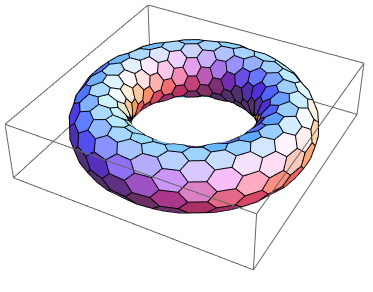
\includegraphics[width=0.75\textwidth]{images/test_image}
	\caption{Comparing Nuclear Fusion and Fission} ~\\
	\small The binding energy per nucleon is what differentiates nuclear fusion from fission. Nuclei heavier than Iron fission (e.g.\ Uranium), while light ones -- such as Hydrogen -- fuse.
	\label{fig:binding_energy}
\end{figure}

\begin{figure}
	\centering
	\begin{adjustbox}{width=0.75\textwidth}
		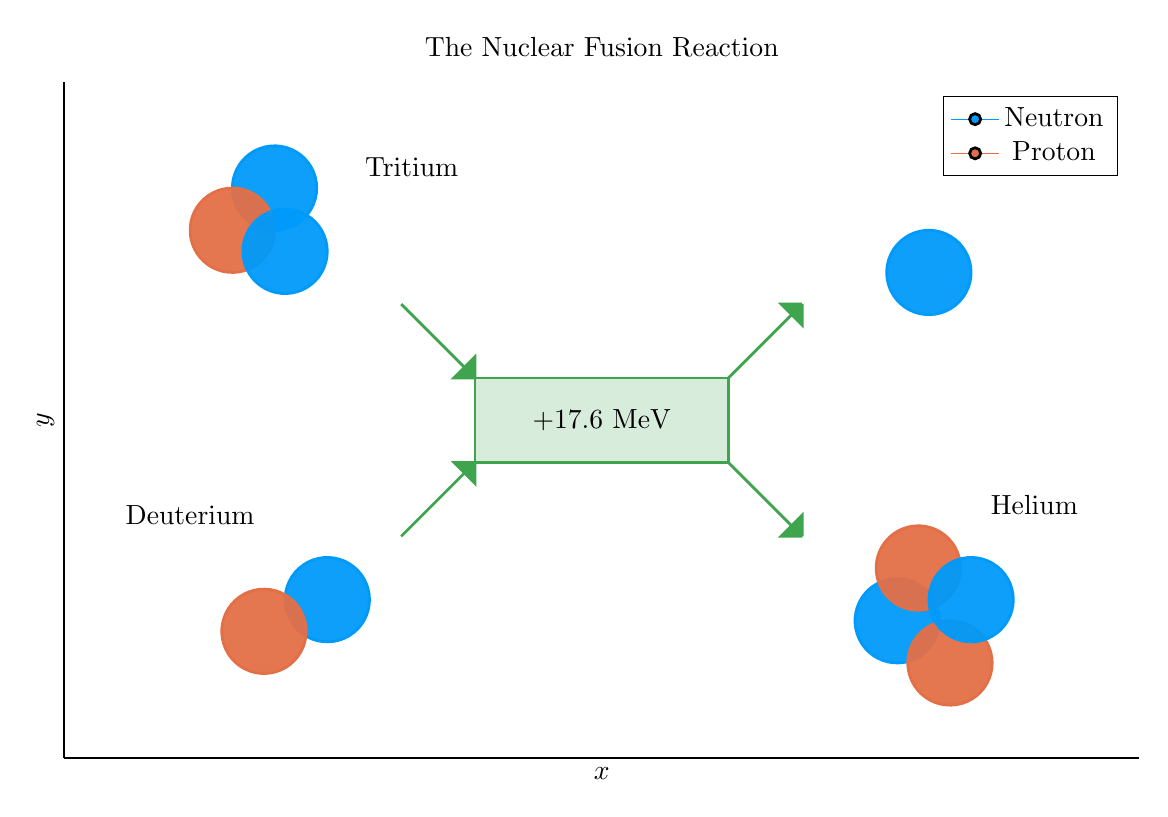
\begin{tikzpicture}[]
\begin{axis}[height = {101.6mm}, axis equal = {true}, ylabel = {$y$}, title = {The Nuclear Fusion Reaction}, xmin = {-12}, xmax = {12}, ymax = {8}, xlabel = {$x$}, {unbounded coords=jump, scaled x ticks = false, xticklabel style={rotate = 0}, xmajorticks=false, xmajorgrids = false, axis lines* = left, scaled y ticks = false, yticklabel style={rotate = 0}, ymajorticks=false, ymajorgrids = false, axis lines* = left,     xshift = 0.0mm,
    yshift = 0.0mm,
    axis background/.style={fill={rgb,1:red,1.00000000;green,1.00000000;blue,1.00000000}}
}, ymin = {-8}, width = {152.4mm}]\addplot+ [color = {rgb,1:red,0.00000000;green,0.60560316;blue,0.97868012},
draw opacity=1.0,
line width=1,
solid,mark = none,
mark size = 2.0,
mark options = {
    color = {rgb,1:red,0.00000000;green,0.00000000;blue,0.00000000}, draw opacity = 1.0,
    fill = {rgb,1:red,0.00000000;green,0.60560316;blue,0.97868012}, fill opacity = 1.0,
    line width = 1,
    rotate = 0,
    solid
},fill = {rgb,1:red,0.00000000;green,0.60560316;blue,0.97868012}, fill opacity=0.95,forget plot]coordinates {
(-6.75, 5.5)
(-6.7582099861767535, 5.627877161684506)
(-6.7827051369609705, 5.7536545839095075)
(-6.823083242653978, 5.875267004879374)
(-6.878681295876611, 5.990717552003938)
(-6.948586378132044, 6.0981105304912155)
(-7.031650649902272, 6.195682550603486)
(-7.126510198141267, 6.2818314824680295)
(-7.231607431689475, 6.355142763005346)
(-7.345216656877606, 6.414412623015813)
(-7.465472413368968, 6.45866785303666)
(-7.590400104966621, 6.48718178341445)
(-7.717948422428345, 6.499486216200688)
(-7.846023025907682, 6.495379112949198)
(-7.972520933956314, 6.4749279121818235)
(-8.095365054421308, 6.438468422049761)
(-8.212538290240834, 6.386599306373)
(-8.32211666012217, 6.320172254596956)
(-8.422300890261317, 6.2402779970753155)
(-8.511445958369134, 6.148228395307789)
(-8.58808810489184, 6.045534901210549)
(-8.650968867902419, 5.933883739117558)
(-8.699055747010668, 5.815108218023621)
(-8.731559156991064, 5.6911586287013725)
(-8.747945392750337, 5.564070219980713)
(-8.747945392750337, 5.435929780019287)
(-8.731559156991064, 5.3088413712986275)
(-8.699055747010668, 5.184891781976379)
(-8.650968867902419, 5.066116260882442)
(-8.58808810489184, 4.954465098789451)
(-8.511445958369135, 4.851771604692212)
(-8.422300890261317, 4.7597220029246845)
(-8.32211666012217, 4.679827745403045)
(-8.212538290240836, 4.613400693627)
(-8.095365054421308, 4.56153157795024)
(-7.972520933956314, 4.5250720878181765)
(-7.846023025907682, 4.504620887050802)
(-7.7179484224283454, 4.500513783799312)
(-7.590400104966621, 4.51281821658555)
(-7.465472413368968, 4.541332146963339)
(-7.345216656877606, 4.585587376984187)
(-7.231607431689476, 4.644857236994653)
(-7.126510198141267, 4.71816851753197)
(-7.031650649902272, 4.804317449396514)
(-6.948586378132044, 4.901889469508784)
(-6.878681295876611, 5.009282447996062)
(-6.823083242653978, 5.124732995120626)
(-6.7827051369609705, 5.2463454160904925)
(-6.7582099861767535, 5.3721228383154935)
(-6.75, 5.5)
};
\addplot+ [color = {rgb,1:red,0.88887350;green,0.43564919;blue,0.27812294},
draw opacity=1.0,
line width=1,
solid,mark = none,
mark size = 2.0,
mark options = {
    color = {rgb,1:red,0.00000000;green,0.00000000;blue,0.00000000}, draw opacity = 1.0,
    fill = {rgb,1:red,0.88887350;green,0.43564919;blue,0.27812294}, fill opacity = 1.0,
    line width = 1,
    rotate = 0,
    solid
},fill = {rgb,1:red,0.88887350;green,0.43564919;blue,0.27812294}, fill opacity=0.95,forget plot]coordinates {
(-7.75, 4.5)
(-7.7582099861767535, 4.627877161684506)
(-7.7827051369609705, 4.7536545839095075)
(-7.823083242653978, 4.875267004879374)
(-7.878681295876611, 4.990717552003938)
(-7.948586378132044, 5.0981105304912155)
(-8.031650649902272, 5.195682550603486)
(-8.126510198141267, 5.2818314824680295)
(-8.231607431689476, 5.355142763005346)
(-8.345216656877605, 5.414412623015813)
(-8.465472413368968, 5.45866785303666)
(-8.590400104966621, 5.48718178341445)
(-8.717948422428345, 5.499486216200688)
(-8.846023025907682, 5.495379112949198)
(-8.972520933956314, 5.4749279121818235)
(-9.095365054421308, 5.438468422049761)
(-9.212538290240834, 5.386599306373)
(-9.32211666012217, 5.320172254596956)
(-9.422300890261317, 5.2402779970753155)
(-9.511445958369134, 5.148228395307789)
(-9.58808810489184, 5.045534901210549)
(-9.650968867902419, 4.933883739117558)
(-9.699055747010668, 4.815108218023621)
(-9.731559156991064, 4.6911586287013725)
(-9.747945392750337, 4.564070219980713)
(-9.747945392750337, 4.435929780019287)
(-9.731559156991064, 4.3088413712986275)
(-9.699055747010668, 4.184891781976379)
(-9.650968867902419, 4.066116260882442)
(-9.58808810489184, 3.9544650987894516)
(-9.511445958369135, 3.8517716046922117)
(-9.422300890261317, 3.7597220029246845)
(-9.32211666012217, 3.6798277454030446)
(-9.212538290240836, 3.613400693627)
(-9.095365054421308, 3.5615315779502397)
(-8.972520933956314, 3.5250720878181765)
(-8.846023025907682, 3.5046208870508018)
(-8.717948422428345, 3.5005137837993123)
(-8.590400104966621, 3.5128182165855497)
(-8.465472413368968, 3.541332146963339)
(-8.345216656877607, 3.5855873769841873)
(-8.231607431689476, 3.6448572369946537)
(-8.126510198141267, 3.71816851753197)
(-8.031650649902272, 3.804317449396514)
(-7.948586378132044, 3.9018894695087836)
(-7.878681295876611, 4.009282447996062)
(-7.823083242653978, 4.124732995120626)
(-7.7827051369609705, 4.2463454160904925)
(-7.7582099861767535, 4.3721228383154935)
(-7.75, 4.5)
};
\addplot+ [color = {rgb,1:red,0.00000000;green,0.60560316;blue,0.97868012},
draw opacity=1.0,
line width=1,
solid,mark = none,
mark size = 2.0,
mark options = {
    color = {rgb,1:red,0.00000000;green,0.00000000;blue,0.00000000}, draw opacity = 1.0,
    fill = {rgb,1:red,0.00000000;green,0.60560316;blue,0.97868012}, fill opacity = 1.0,
    line width = 1,
    rotate = 0,
    solid
},fill = {rgb,1:red,0.00000000;green,0.60560316;blue,0.97868012}, fill opacity=0.95,forget plot]coordinates {
(-6.5, 4.0)
(-6.5082099861767535, 4.127877161684506)
(-6.5327051369609705, 4.2536545839095075)
(-6.573083242653978, 4.375267004879374)
(-6.628681295876611, 4.490717552003938)
(-6.698586378132044, 4.5981105304912155)
(-6.781650649902272, 4.695682550603486)
(-6.876510198141267, 4.7818314824680295)
(-6.981607431689475, 4.855142763005346)
(-7.095216656877606, 4.914412623015813)
(-7.215472413368968, 4.95866785303666)
(-7.340400104966621, 4.98718178341445)
(-7.467948422428345, 4.999486216200688)
(-7.596023025907682, 4.995379112949198)
(-7.722520933956314, 4.9749279121818235)
(-7.845365054421308, 4.938468422049761)
(-7.962538290240835, 4.886599306373)
(-8.07211666012217, 4.820172254596956)
(-8.172300890261317, 4.7402779970753155)
(-8.261445958369134, 4.648228395307789)
(-8.33808810489184, 4.545534901210549)
(-8.400968867902419, 4.433883739117558)
(-8.449055747010668, 4.315108218023621)
(-8.481559156991064, 4.1911586287013725)
(-8.497945392750337, 4.064070219980713)
(-8.497945392750337, 3.935929780019287)
(-8.481559156991064, 3.8088413712986275)
(-8.449055747010668, 3.6848917819763796)
(-8.400968867902419, 3.566116260882442)
(-8.33808810489184, 3.4544650987894516)
(-8.261445958369135, 3.3517716046922117)
(-8.172300890261317, 3.2597220029246845)
(-8.07211666012217, 3.1798277454030446)
(-7.962538290240835, 3.113400693627)
(-7.8453650544213085, 3.0615315779502397)
(-7.722520933956314, 3.0250720878181765)
(-7.596023025907682, 3.0046208870508018)
(-7.4679484224283454, 3.0005137837993123)
(-7.340400104966621, 3.0128182165855497)
(-7.215472413368968, 3.041332146963339)
(-7.095216656877606, 3.0855873769841873)
(-6.981607431689476, 3.1448572369946537)
(-6.876510198141267, 3.21816851753197)
(-6.781650649902272, 3.304317449396514)
(-6.698586378132044, 3.4018894695087836)
(-6.628681295876611, 3.5092824479960623)
(-6.573083242653978, 3.6247329951206253)
(-6.5327051369609705, 3.7463454160904925)
(-6.5082099861767535, 3.8721228383154935)
(-6.5, 3.9999999999999996)
};
\addplot+ [color = {rgb,1:red,0.00000000;green,0.60560316;blue,0.97868012},
draw opacity=1.0,
line width=1,
solid,mark = none,
mark size = 2.0,
mark options = {
    color = {rgb,1:red,0.00000000;green,0.00000000;blue,0.00000000}, draw opacity = 1.0,
    fill = {rgb,1:red,0.00000000;green,0.60560316;blue,0.97868012}, fill opacity = 1.0,
    line width = 1,
    rotate = 0,
    solid
},fill = {rgb,1:red,0.00000000;green,0.60560316;blue,0.97868012}, fill opacity=0.95,forget plot]coordinates {
(-5.5, -4.25)
(-5.5082099861767535, -4.122122838315494)
(-5.5327051369609705, -3.9963454160904925)
(-5.573083242653978, -3.8747329951206257)
(-5.628681295876611, -3.7592824479960623)
(-5.698586378132044, -3.651889469508784)
(-5.781650649902272, -3.5543174493965135)
(-5.876510198141267, -3.46816851753197)
(-5.981607431689475, -3.394857236994654)
(-6.095216656877606, -3.3355873769841873)
(-6.215472413368968, -3.2913321469633394)
(-6.340400104966621, -3.2628182165855497)
(-6.467948422428345, -3.2505137837993123)
(-6.596023025907682, -3.2546208870508018)
(-6.722520933956314, -3.2750720878181765)
(-6.845365054421308, -3.3115315779502397)
(-6.962538290240835, -3.363400693627)
(-7.07211666012217, -3.429827745403044)
(-7.172300890261317, -3.5097220029246845)
(-7.261445958369134, -3.6017716046922117)
(-7.338088104891841, -3.704465098789451)
(-7.400968867902419, -3.816116260882442)
(-7.449055747010669, -3.934891781976379)
(-7.481559156991065, -4.0588413712986275)
(-7.497945392750337, -4.185929780019287)
(-7.497945392750337, -4.314070219980713)
(-7.481559156991065, -4.4411586287013725)
(-7.449055747010669, -4.565108218023621)
(-7.400968867902419, -4.683883739117558)
(-7.338088104891841, -4.795534901210549)
(-7.261445958369134, -4.898228395307788)
(-7.172300890261317, -4.9902779970753155)
(-7.07211666012217, -5.070172254596955)
(-6.962538290240835, -5.136599306373)
(-6.8453650544213085, -5.18846842204976)
(-6.722520933956314, -5.2249279121818235)
(-6.596023025907682, -5.245379112949198)
(-6.4679484224283454, -5.249486216200688)
(-6.340400104966621, -5.23718178341445)
(-6.215472413368968, -5.208667853036661)
(-6.095216656877606, -5.164412623015813)
(-5.981607431689476, -5.105142763005347)
(-5.876510198141267, -5.03183148246803)
(-5.781650649902272, -4.945682550603486)
(-5.698586378132044, -4.848110530491216)
(-5.628681295876611, -4.740717552003938)
(-5.573083242653978, -4.625267004879374)
(-5.5327051369609705, -4.5036545839095075)
(-5.5082099861767535, -4.3778771616845065)
(-5.5, -4.25)
};
\addplot+ [color = {rgb,1:red,0.88887350;green,0.43564919;blue,0.27812294},
draw opacity=1.0,
line width=1,
solid,mark = none,
mark size = 2.0,
mark options = {
    color = {rgb,1:red,0.00000000;green,0.00000000;blue,0.00000000}, draw opacity = 1.0,
    fill = {rgb,1:red,0.88887350;green,0.43564919;blue,0.27812294}, fill opacity = 1.0,
    line width = 1,
    rotate = 0,
    solid
},fill = {rgb,1:red,0.88887350;green,0.43564919;blue,0.27812294}, fill opacity=0.95,forget plot]coordinates {
(-7.0, -5.0)
(-7.0082099861767535, -4.872122838315494)
(-7.0327051369609705, -4.7463454160904925)
(-7.073083242653978, -4.624732995120626)
(-7.128681295876611, -4.509282447996062)
(-7.198586378132044, -4.4018894695087845)
(-7.281650649902272, -4.304317449396514)
(-7.376510198141267, -4.2181685175319705)
(-7.481607431689475, -4.144857236994654)
(-7.595216656877606, -4.085587376984187)
(-7.715472413368968, -4.04133214696334)
(-7.840400104966621, -4.01281821658555)
(-7.967948422428345, -4.000513783799312)
(-8.096023025907682, -4.004620887050802)
(-8.222520933956314, -4.0250720878181765)
(-8.345365054421308, -4.061531577950239)
(-8.462538290240834, -4.113400693627)
(-8.57211666012217, -4.179827745403044)
(-8.672300890261317, -4.2597220029246845)
(-8.761445958369134, -4.351771604692211)
(-8.83808810489184, -4.454465098789451)
(-8.900968867902419, -4.566116260882442)
(-8.949055747010668, -4.684891781976379)
(-8.981559156991064, -4.8088413712986275)
(-8.997945392750337, -4.935929780019287)
(-8.997945392750337, -5.064070219980713)
(-8.981559156991064, -5.1911586287013725)
(-8.949055747010668, -5.315108218023621)
(-8.900968867902419, -5.433883739117558)
(-8.83808810489184, -5.545534901210549)
(-8.761445958369135, -5.648228395307788)
(-8.672300890261317, -5.7402779970753155)
(-8.57211666012217, -5.820172254596955)
(-8.462538290240836, -5.886599306373)
(-8.345365054421308, -5.93846842204976)
(-8.222520933956314, -5.9749279121818235)
(-8.096023025907682, -5.995379112949198)
(-7.9679484224283454, -5.999486216200688)
(-7.840400104966621, -5.98718178341445)
(-7.715472413368968, -5.958667853036661)
(-7.595216656877606, -5.914412623015813)
(-7.481607431689476, -5.855142763005347)
(-7.376510198141267, -5.78183148246803)
(-7.281650649902272, -5.695682550603486)
(-7.198586378132044, -5.598110530491216)
(-7.128681295876611, -5.490717552003938)
(-7.073083242653978, -5.375267004879374)
(-7.0327051369609705, -5.2536545839095075)
(-7.0082099861767535, -5.1278771616845065)
(-7.0, -5.0)
};
\addplot+ [color = {rgb,1:red,0.24222430;green,0.64327509;blue,0.30444865},
draw opacity=1.0,
line width=1,
solid,mark = none,
mark size = 2.0,
mark options = {
    color = {rgb,1:red,0.00000000;green,0.00000000;blue,0.00000000}, draw opacity = 1.0,
    fill = {rgb,1:red,0.24222430;green,0.64327509;blue,0.30444865}, fill opacity = 1.0,
    line width = 1,
    rotate = 0,
    solid
},forget plot]coordinates {
(-4.75, 2.75)
(-3.0, 1.0)
};
\addplot+ [color = {rgb,1:red,0.24222430;green,0.64327509;blue,0.30444865},
draw opacity=1.0,
line width=1,
solid,mark = none,
mark size = 2.0,
mark options = {
    color = {rgb,1:red,0.00000000;green,0.00000000;blue,0.00000000}, draw opacity = 1.0,
    fill = {rgb,1:red,0.24222430;green,0.64327509;blue,0.30444865}, fill opacity = 1.0,
    line width = 1,
    rotate = 0,
    solid
},forget plot]coordinates {
(-4.75, -2.75)
(-3.0, -1.0)
};
\addplot+ [color = {rgb,1:red,0.24222430;green,0.64327509;blue,0.30444865},
draw opacity=1.0,
line width=1,
solid,mark = none,
mark size = 2.0,
mark options = {
    color = {rgb,1:red,0.00000000;green,0.00000000;blue,0.00000000}, draw opacity = 1.0,
    fill = {rgb,1:red,0.24222430;green,0.64327509;blue,0.30444865}, fill opacity = 1.0,
    line width = 1,
    rotate = 0,
    solid
},fill = {rgb,1:red,0.24222430;green,0.64327509;blue,0.30444865}, fill opacity=1.0,forget plot]coordinates {
(-3.0, 1.0)
(-3.5, 1.0)
(-3.0, 1.5)
(-3.0, 1.0)
};
\addplot+ [color = {rgb,1:red,0.24222430;green,0.64327509;blue,0.30444865},
draw opacity=1.0,
line width=1,
solid,mark = none,
mark size = 2.0,
mark options = {
    color = {rgb,1:red,0.00000000;green,0.00000000;blue,0.00000000}, draw opacity = 1.0,
    fill = {rgb,1:red,0.24222430;green,0.64327509;blue,0.30444865}, fill opacity = 1.0,
    line width = 1,
    rotate = 0,
    solid
},fill = {rgb,1:red,0.24222430;green,0.64327509;blue,0.30444865}, fill opacity=1.0,forget plot]coordinates {
(-3.0, -1.0)
(-3.5, -1.0)
(-3.0, -1.5)
(-3.0, -1.0)
};
\addplot+ [color = {rgb,1:red,0.24222430;green,0.64327509;blue,0.30444865},
draw opacity=1.0,
line width=1,
solid,mark = none,
mark size = 2.0,
mark options = {
    color = {rgb,1:red,0.00000000;green,0.00000000;blue,0.00000000}, draw opacity = 1.0,
    fill = {rgb,1:red,0.24222430;green,0.64327509;blue,0.30444865}, fill opacity = 1.0,
    line width = 1,
    rotate = 0,
    solid
},forget plot]coordinates {
(3.0, 1.0)
(4.75, 2.75)
};
\addplot+ [color = {rgb,1:red,0.24222430;green,0.64327509;blue,0.30444865},
draw opacity=1.0,
line width=1,
solid,mark = none,
mark size = 2.0,
mark options = {
    color = {rgb,1:red,0.00000000;green,0.00000000;blue,0.00000000}, draw opacity = 1.0,
    fill = {rgb,1:red,0.24222430;green,0.64327509;blue,0.30444865}, fill opacity = 1.0,
    line width = 1,
    rotate = 0,
    solid
},forget plot]coordinates {
(3.0, -1.0)
(4.75, -2.75)
};
\addplot+ [color = {rgb,1:red,0.24222430;green,0.64327509;blue,0.30444865},
draw opacity=1.0,
line width=1,
solid,mark = none,
mark size = 2.0,
mark options = {
    color = {rgb,1:red,0.00000000;green,0.00000000;blue,0.00000000}, draw opacity = 1.0,
    fill = {rgb,1:red,0.24222430;green,0.64327509;blue,0.30444865}, fill opacity = 1.0,
    line width = 1,
    rotate = 0,
    solid
},fill = {rgb,1:red,0.24222430;green,0.64327509;blue,0.30444865}, fill opacity=1.0,forget plot]coordinates {
(4.75, 2.75)
(4.25, 2.75)
(4.75, 2.25)
(4.75, 2.75)
};
\addplot+ [color = {rgb,1:red,0.24222430;green,0.64327509;blue,0.30444865},
draw opacity=1.0,
line width=1,
solid,mark = none,
mark size = 2.0,
mark options = {
    color = {rgb,1:red,0.00000000;green,0.00000000;blue,0.00000000}, draw opacity = 1.0,
    fill = {rgb,1:red,0.24222430;green,0.64327509;blue,0.30444865}, fill opacity = 1.0,
    line width = 1,
    rotate = 0,
    solid
},fill = {rgb,1:red,0.24222430;green,0.64327509;blue,0.30444865}, fill opacity=1.0,forget plot]coordinates {
(4.75, -2.75)
(4.25, -2.75)
(4.75, -2.25)
(4.75, -2.75)
};
\addplot+ [color = {rgb,1:red,0.24222430;green,0.64327509;blue,0.30444865},
draw opacity=1.0,
line width=1,
solid,mark = none,
mark size = 2.0,
mark options = {
    color = {rgb,1:red,0.00000000;green,0.00000000;blue,0.00000000}, draw opacity = 1.0,
    fill = {rgb,1:red,0.24222430;green,0.64327509;blue,0.30444865}, fill opacity = 1.0,
    line width = 1,
    rotate = 0,
    solid
},fill = {rgb,1:red,0.24222430;green,0.64327509;blue,0.30444865}, fill opacity=0.2,forget plot]coordinates {
(-3, 1)
(3, 1)
(3, -1)
(-3, -1)
(-3, 1)
};
\addplot+ [color = {rgb,1:red,0.00000000;green,0.60560316;blue,0.97868012},
draw opacity=1.0,
line width=1,
solid,mark = none,
mark size = 2.0,
mark options = {
    color = {rgb,1:red,0.00000000;green,0.00000000;blue,0.00000000}, draw opacity = 1.0,
    fill = {rgb,1:red,0.00000000;green,0.60560316;blue,0.97868012}, fill opacity = 1.0,
    line width = 1,
    rotate = 0,
    solid
},fill = {rgb,1:red,0.00000000;green,0.60560316;blue,0.97868012}, fill opacity=0.95,forget plot]coordinates {
(8.75, 3.5)
(8.741790013823246, 3.627877161684506)
(8.71729486303903, 3.7536545839095075)
(8.67691675734602, 3.8752670048793743)
(8.62131870412339, 3.9907175520039377)
(8.551413621867956, 4.0981105304912155)
(8.468349350097728, 4.195682550603486)
(8.373489801858733, 4.2818314824680295)
(8.268392568310524, 4.355142763005346)
(8.154783343122395, 4.414412623015813)
(8.034527586631032, 4.45866785303666)
(7.909599895033379, 4.48718178341445)
(7.782051577571655, 4.499486216200688)
(7.653976974092318, 4.495379112949198)
(7.527479066043686, 4.4749279121818235)
(7.404634945578692, 4.438468422049761)
(7.287461709759165, 4.386599306373)
(7.17788333987783, 4.320172254596956)
(7.077699109738683, 4.2402779970753155)
(6.988554041630866, 4.148228395307789)
(6.911911895108159, 4.045534901210549)
(6.849031132097581, 3.933883739117558)
(6.800944252989331, 3.815108218023621)
(6.768440843008935, 3.6911586287013725)
(6.752054607249663, 3.5640702199807133)
(6.752054607249663, 3.435929780019287)
(6.768440843008935, 3.3088413712986275)
(6.800944252989331, 3.1848917819763796)
(6.849031132097581, 3.066116260882442)
(6.911911895108159, 2.9544650987894516)
(6.988554041630866, 2.8517716046922117)
(7.077699109738683, 2.7597220029246845)
(7.17788333987783, 2.6798277454030446)
(7.287461709759165, 2.613400693627)
(7.4046349455786915, 2.5615315779502397)
(7.527479066043686, 2.5250720878181765)
(7.653976974092318, 2.5046208870508018)
(7.7820515775716546, 2.5005137837993123)
(7.909599895033379, 2.5128182165855497)
(8.034527586631032, 2.541332146963339)
(8.154783343122393, 2.5855873769841873)
(8.268392568310524, 2.6448572369946537)
(8.373489801858733, 2.71816851753197)
(8.468349350097728, 2.804317449396514)
(8.551413621867956, 2.9018894695087836)
(8.62131870412339, 3.0092824479960623)
(8.67691675734602, 3.1247329951206253)
(8.71729486303903, 3.2463454160904925)
(8.741790013823246, 3.3721228383154935)
(8.75, 3.4999999999999996)
};
\addplot+ [color = {rgb,1:red,0.00000000;green,0.60560316;blue,0.97868012},
draw opacity=1.0,
line width=1,
solid,mark = none,
mark size = 2.0,
mark options = {
    color = {rgb,1:red,0.00000000;green,0.00000000;blue,0.00000000}, draw opacity = 1.0,
    fill = {rgb,1:red,0.00000000;green,0.60560316;blue,0.97868012}, fill opacity = 1.0,
    line width = 1,
    rotate = 0,
    solid
},fill = {rgb,1:red,0.00000000;green,0.60560316;blue,0.97868012}, fill opacity=0.95,forget plot]coordinates {
(8.0, -4.75)
(7.9917900138232465, -4.622122838315494)
(7.9672948630390295, -4.4963454160904925)
(7.926916757346022, -4.374732995120626)
(7.871318704123389, -4.259282447996062)
(7.801413621867956, -4.1518894695087845)
(7.718349350097728, -4.054317449396514)
(7.623489801858733, -3.96816851753197)
(7.518392568310525, -3.894857236994654)
(7.404783343122394, -3.8355873769841873)
(7.284527586631032, -3.7913321469633394)
(7.159599895033379, -3.7628182165855497)
(7.032051577571655, -3.7505137837993123)
(6.903976974092318, -3.7546208870508018)
(6.777479066043686, -3.7750720878181765)
(6.654634945578692, -3.8115315779502397)
(6.537461709759165, -3.863400693627)
(6.42788333987783, -3.929827745403044)
(6.327699109738683, -4.0097220029246845)
(6.238554041630866, -4.101771604692211)
(6.161911895108159, -4.204465098789451)
(6.099031132097581, -4.316116260882442)
(6.050944252989331, -4.434891781976379)
(6.018440843008935, -4.5588413712986275)
(6.002054607249663, -4.685929780019287)
(6.002054607249663, -4.814070219980713)
(6.018440843008935, -4.9411586287013725)
(6.050944252989331, -5.065108218023621)
(6.099031132097581, -5.183883739117558)
(6.161911895108159, -5.295534901210549)
(6.238554041630866, -5.398228395307788)
(6.327699109738683, -5.4902779970753155)
(6.42788333987783, -5.570172254596955)
(6.537461709759165, -5.636599306373)
(6.6546349455786915, -5.68846842204976)
(6.777479066043686, -5.7249279121818235)
(6.903976974092318, -5.745379112949198)
(7.0320515775716546, -5.749486216200688)
(7.159599895033379, -5.73718178341445)
(7.284527586631032, -5.708667853036661)
(7.404783343122394, -5.664412623015813)
(7.518392568310524, -5.605142763005347)
(7.623489801858733, -5.53183148246803)
(7.718349350097728, -5.445682550603486)
(7.801413621867956, -5.348110530491216)
(7.871318704123389, -5.240717552003938)
(7.926916757346022, -5.125267004879374)
(7.9672948630390295, -5.0036545839095075)
(7.9917900138232465, -4.8778771616845065)
(8.0, -4.75)
};
\addplot+ [color = {rgb,1:red,0.88887350;green,0.43564919;blue,0.27812294},
draw opacity=1.0,
line width=1,
solid,mark = none,
mark size = 2.0,
mark options = {
    color = {rgb,1:red,0.00000000;green,0.00000000;blue,0.00000000}, draw opacity = 1.0,
    fill = {rgb,1:red,0.88887350;green,0.43564919;blue,0.27812294}, fill opacity = 1.0,
    line width = 1,
    rotate = 0,
    solid
},fill = {rgb,1:red,0.88887350;green,0.43564919;blue,0.27812294}, fill opacity=0.95,forget plot]coordinates {
(9.25, -5.75)
(9.241790013823246, -5.622122838315494)
(9.21729486303903, -5.4963454160904925)
(9.17691675734602, -5.374732995120626)
(9.12131870412339, -5.259282447996062)
(9.051413621867956, -5.1518894695087845)
(8.968349350097728, -5.054317449396514)
(8.873489801858733, -4.9681685175319705)
(8.768392568310524, -4.894857236994654)
(8.654783343122395, -4.835587376984187)
(8.534527586631032, -4.79133214696334)
(8.409599895033379, -4.76281821658555)
(8.282051577571655, -4.750513783799312)
(8.153976974092318, -4.754620887050802)
(8.027479066043686, -4.7750720878181765)
(7.904634945578692, -4.811531577950239)
(7.787461709759165, -4.863400693627)
(7.67788333987783, -4.929827745403044)
(7.577699109738683, -5.0097220029246845)
(7.488554041630866, -5.101771604692211)
(7.411911895108159, -5.204465098789451)
(7.349031132097581, -5.316116260882442)
(7.300944252989331, -5.434891781976379)
(7.268440843008935, -5.5588413712986275)
(7.252054607249663, -5.685929780019287)
(7.252054607249663, -5.814070219980713)
(7.268440843008935, -5.9411586287013725)
(7.300944252989331, -6.065108218023621)
(7.349031132097581, -6.183883739117558)
(7.411911895108159, -6.295534901210549)
(7.488554041630866, -6.398228395307788)
(7.577699109738683, -6.4902779970753155)
(7.67788333987783, -6.570172254596955)
(7.787461709759165, -6.636599306373)
(7.9046349455786915, -6.68846842204976)
(8.027479066043686, -6.7249279121818235)
(8.153976974092318, -6.745379112949198)
(8.282051577571655, -6.749486216200688)
(8.409599895033379, -6.73718178341445)
(8.534527586631032, -6.708667853036661)
(8.654783343122393, -6.664412623015813)
(8.768392568310524, -6.605142763005347)
(8.873489801858733, -6.53183148246803)
(8.968349350097728, -6.445682550603486)
(9.051413621867956, -6.348110530491216)
(9.12131870412339, -6.240717552003938)
(9.17691675734602, -6.125267004879374)
(9.21729486303903, -6.0036545839095075)
(9.241790013823246, -5.8778771616845065)
(9.25, -5.75)
};
\addplot+ [color = {rgb,1:red,0.88887350;green,0.43564919;blue,0.27812294},
draw opacity=1.0,
line width=1,
solid,mark = none,
mark size = 2.0,
mark options = {
    color = {rgb,1:red,0.00000000;green,0.00000000;blue,0.00000000}, draw opacity = 1.0,
    fill = {rgb,1:red,0.88887350;green,0.43564919;blue,0.27812294}, fill opacity = 1.0,
    line width = 1,
    rotate = 0,
    solid
},fill = {rgb,1:red,0.88887350;green,0.43564919;blue,0.27812294}, fill opacity=0.95,forget plot]coordinates {
(8.5, -3.5)
(8.491790013823246, -3.372122838315494)
(8.46729486303903, -3.2463454160904925)
(8.42691675734602, -3.1247329951206257)
(8.37131870412339, -3.0092824479960623)
(8.301413621867956, -2.901889469508784)
(8.218349350097728, -2.8043174493965135)
(8.123489801858733, -2.71816851753197)
(8.018392568310524, -2.644857236994654)
(7.904783343122394, -2.5855873769841873)
(7.784527586631032, -2.5413321469633394)
(7.659599895033379, -2.5128182165855497)
(7.532051577571655, -2.5005137837993123)
(7.403976974092318, -2.5046208870508018)
(7.277479066043686, -2.5250720878181765)
(7.154634945578692, -2.5615315779502397)
(7.037461709759165, -2.613400693627)
(6.92788333987783, -2.679827745403044)
(6.827699109738683, -2.7597220029246845)
(6.738554041630866, -2.8517716046922117)
(6.661911895108159, -2.954465098789451)
(6.599031132097581, -3.066116260882442)
(6.550944252989331, -3.184891781976379)
(6.518440843008935, -3.3088413712986275)
(6.502054607249663, -3.4359297800192867)
(6.502054607249663, -3.564070219980713)
(6.518440843008935, -3.6911586287013725)
(6.550944252989331, -3.8151082180236204)
(6.599031132097581, -3.933883739117558)
(6.661911895108159, -4.045534901210549)
(6.738554041630866, -4.148228395307788)
(6.827699109738683, -4.2402779970753155)
(6.92788333987783, -4.320172254596955)
(7.037461709759165, -4.386599306373)
(7.1546349455786915, -4.43846842204976)
(7.277479066043686, -4.4749279121818235)
(7.403976974092318, -4.495379112949198)
(7.5320515775716546, -4.499486216200688)
(7.659599895033379, -4.48718178341445)
(7.784527586631032, -4.458667853036661)
(7.904783343122394, -4.414412623015813)
(8.018392568310524, -4.355142763005347)
(8.123489801858733, -4.28183148246803)
(8.218349350097728, -4.195682550603486)
(8.301413621867956, -4.098110530491216)
(8.37131870412339, -3.9907175520039377)
(8.42691675734602, -3.8752670048793747)
(8.46729486303903, -3.7536545839095075)
(8.491790013823246, -3.6278771616845065)
(8.5, -3.5000000000000004)
};
\addplot+ [color = {rgb,1:red,0.00000000;green,0.60560316;blue,0.97868012},
draw opacity=1.0,
line width=1,
solid,mark = none,
mark size = 2.0,
mark options = {
    color = {rgb,1:red,0.00000000;green,0.00000000;blue,0.00000000}, draw opacity = 1.0,
    fill = {rgb,1:red,0.00000000;green,0.60560316;blue,0.97868012}, fill opacity = 1.0,
    line width = 1,
    rotate = 0,
    solid
},fill = {rgb,1:red,0.00000000;green,0.60560316;blue,0.97868012}, fill opacity=0.95,forget plot]coordinates {
(9.75, -4.25)
(9.741790013823246, -4.122122838315494)
(9.71729486303903, -3.9963454160904925)
(9.67691675734602, -3.8747329951206257)
(9.62131870412339, -3.7592824479960623)
(9.551413621867956, -3.651889469508784)
(9.468349350097728, -3.5543174493965135)
(9.373489801858733, -3.46816851753197)
(9.268392568310524, -3.394857236994654)
(9.154783343122395, -3.3355873769841873)
(9.034527586631032, -3.2913321469633394)
(8.909599895033379, -3.2628182165855497)
(8.782051577571655, -3.2505137837993123)
(8.653976974092318, -3.2546208870508018)
(8.527479066043686, -3.2750720878181765)
(8.404634945578692, -3.3115315779502397)
(8.287461709759166, -3.363400693627)
(8.17788333987783, -3.429827745403044)
(8.077699109738683, -3.5097220029246845)
(7.988554041630866, -3.6017716046922117)
(7.911911895108159, -3.704465098789451)
(7.849031132097581, -3.816116260882442)
(7.800944252989331, -3.934891781976379)
(7.768440843008935, -4.0588413712986275)
(7.752054607249663, -4.185929780019287)
(7.752054607249663, -4.314070219980713)
(7.768440843008935, -4.4411586287013725)
(7.800944252989331, -4.565108218023621)
(7.849031132097581, -4.683883739117558)
(7.911911895108159, -4.795534901210549)
(7.988554041630866, -4.898228395307788)
(8.077699109738683, -4.9902779970753155)
(8.17788333987783, -5.070172254596955)
(8.287461709759164, -5.136599306373)
(8.404634945578692, -5.18846842204976)
(8.527479066043686, -5.2249279121818235)
(8.653976974092318, -5.245379112949198)
(8.782051577571655, -5.249486216200688)
(8.909599895033379, -5.23718178341445)
(9.034527586631032, -5.208667853036661)
(9.154783343122393, -5.164412623015813)
(9.268392568310524, -5.105142763005347)
(9.373489801858733, -5.03183148246803)
(9.468349350097728, -4.945682550603486)
(9.551413621867956, -4.848110530491216)
(9.62131870412339, -4.740717552003938)
(9.67691675734602, -4.625267004879374)
(9.71729486303903, -4.5036545839095075)
(9.741790013823246, -4.3778771616845065)
(9.75, -4.25)
};
\addplot+[draw=none, color = {rgb,1:red,0.00000000;green,0.60560316;blue,0.97868012},
draw opacity=1.0,
line width=0,
solid,mark = *,
mark size = 2.0,
mark options = {
    color = {rgb,1:red,0.00000000;green,0.00000000;blue,0.00000000}, draw opacity = 1.0,
    fill = {rgb,1:red,0.00000000;green,0.60560316;blue,0.97868012}, fill opacity = 1.0,
    line width = 1,
    rotate = 0,
    solid
}] coordinates {
(100, 100)
};
\addlegendentry{Neutron}
\addplot+[draw=none, color = {rgb,1:red,0.88887350;green,0.43564919;blue,0.27812294},
draw opacity=1.0,
line width=0,
solid,mark = *,
mark size = 2.0,
mark options = {
    color = {rgb,1:red,0.00000000;green,0.00000000;blue,0.00000000}, draw opacity = 1.0,
    fill = {rgb,1:red,0.88887350;green,0.43564919;blue,0.27812294}, fill opacity = 1.0,
    line width = 1,
    rotate = 0,
    solid
}] coordinates {
(100, 100)
};
\addlegendentry{Proton}
\node at (axis cs:-4.5, 6) [,
color={rgb,1:red,0.00000000;green,0.00000000;blue,0.00000000}, draw opacity=1.0,
rotate=0.0
] {Tritium};
\node at (axis cs:-9.75, -2.25) [,
color={rgb,1:red,0.00000000;green,0.00000000;blue,0.00000000}, draw opacity=1.0,
rotate=0.0
] {Deuterium};
\node at (axis cs:0, 0) [,
color={rgb,1:red,0.00000000;green,0.00000000;blue,0.00000000}, draw opacity=1.0,
rotate=0.0
] {+17.6 MeV};
\node at (axis cs:10.25, -2) [,
color={rgb,1:red,0.00000000;green,0.00000000;blue,0.00000000}, draw opacity=1.0,
rotate=0.0
] {Helium};
\end{axis}

\end{tikzpicture}

	\end{adjustbox}
%	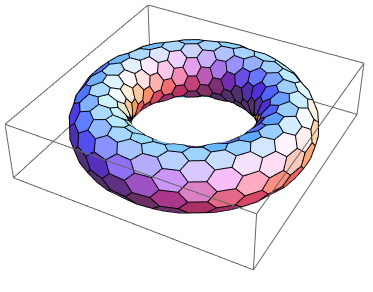
\includegraphics[width=0.75\textwidth]{images/test_image}
	\caption{The D-T Fusion Reaction} ~\\
	\small In a first generation tokamak reactor, the main source of energy will come from two hydrogen isotopes fusing into a helium particle -- and ejecting a 14.1 MeV neutron.
	\label{fig:fusion_reaction}
\end{figure}

What this reaction (shown in \cref{fig:fusion_reaction}) describes is two isotopes of hydrogen -- i.e.\ deuterium and tritium -- fusing into a heavier element, helium, while simultaneously ejecting a neutron. The entire energy of the fusion reaction ($E_F$) is then divvied up 80-20 between the neutron and helium, respectively. Quantitatively, the helium (often referred to as an alpha particle) receives 3.5 MeV.
\begin{equation}
	P_n = 0.8 \cdot P_F
	\label{eq:p_n}
\end{equation}
\myequations{Neutron Power -- $P_n$}
\begin{equation}
	P_\alpha = 0.2 \cdot P_F
	\label{eq:palpha}
\end{equation}
\myequations{Alpha Power -- $P_\alpha$}
The final point to make is the main difference between the two fusion products: helium (i.e.\ the alpha particle) and the neutron. First, neutrons lack a charge -- they are neutral. This means they cannot be confined with magnetic fields. As such, they simply move in straight lines until they collide with other particles. As the structure of a tokamak is mainly metal, the neutron is much more likely to collide there than the gaseous plasma, which is orders of magnitude less dense. Conversely, alpha particles are charged -- when stripped of their electrons -- and can therefore be kept within the plasma using magnets. What this means practically is that of the 17.6 MeV that comes from every fusion reaction, only 3.5 MeV remains inside the plasma (within the helium particle species).

\section{Bosch-Hale Reactivity}

The formula for fusion power used in this model makes use of a reactivity term -- $(\sigma v)$:\cite{jeff}
\begin{equation}
	P_F = \int E_F \, n_D \, n_T \, \langle \sigma v \rangle \, d \textbf{r}
\end{equation}

Summarizing the work of \cref{subsection:fusion_derive}, this fusion power volume integral can be reduced to a 0-D form -- assuming the geometry prescribed by this model:
\begin{equation}
	P_F = K_F \cdot ( \, \overline{n}^2 \, R_0^3 \, ) \cdot (\sigma v) \ \ \ [MW]
\end{equation}
\begin{equation}
	 (\sigma v) = 10^{21} \, (1+\nu_n)^2 \int\limits_0^1 ( 1 - \rho^2 ) ^ { \, 2 \nu_n} \langle \sigma v \rangle \, \rho \, d\rho
\end{equation}
\begin{equation}
	K_F = 278.3 \, ( f_D^2 \, \epsilon^2 \kappa \, g )
\end{equation}

This reactivity term (or volumetric fusion reaction rate) can then be approximated by the Bosch-Hale parameterization, with coefficients given in \cref{table:rrParam}.\cite{boschhale,zach}
\begin{equation}
	\tcboxmath{
	\langle \sigma v \rangle = C_1 \cdot \theta \cdot \textnormal{exp}(-3 \xi) \cdot \sqrt{ \frac{\xi  }{m_\mu  c^2 T^3} }  \ \ \, [ \, \sfrac{ \textnormal{m}^3 }{ \textnormal{s} } \, ] }
\end{equation}
\begin{equation}
	\theta = T \cdot \left(1-\frac{T(C_2+T(C_4+TC_6))}{1+T(C_3+T(C_5+TC_7))}\right) ^{-1}
\end{equation}
\begin{equation}
	\xi = \left(\frac{B_G^2}{4\theta}\right)^{1/3}
\end{equation}

For D-T (Deuterium-Tritium) fuel within a standard fusion temperature regime (i.e. $T \in [10, 20]$ keV), this can be simplified to:\cite{zach}
\begin{equation}
		\langle\sigma v\rangle_\mathrm{DT} = 1.1\times10^{-24} \cdot  \, T^2   \ \ \ [ \, \sfrac{ \textnormal{m}^3 }{ \textnormal{s} } \, ]
\end{equation}
In our model, each appearance of T is set to the radial profile defined earlier -- as it appears inside an integral.

Example tabulations for this reactivity are given in \cref{table:rr}.\cite{zach,nrl,boschhale}

\begin{table}[h!]\small
  \noindent
  \centering
  \caption{Bosch-Hale Parametrization Coefficients}
  \begin{tabular}{c | c c | c | c}
    \multicolumn{5}{c}{}\\
    \hline
    & $^2$H(d,n)$^3$He & $^2$H(d,p)$^3$H & $^3H$(d,n)$^4$He & $^3$He(d,p)$^4$He\\
    \hline\hline
    B$_G$ [keV$^{1/2}$] & 31.3970 & 31.3970 & 34.3827   & 68.7508 \\
    $m_\mu c^2$ [keV]   & 937 814 & 937 814 & 1 124 656 & 1 124 572 \\
    \hline
            % 2H(d,n)                    % 2H(d,p)                   % 3H(d,n)                    % 3He(d,p)
    C$_1$& 5.43360$\times$10$^{-12}$  & 5.65718$\times$10$^{-12}$ & 1.17302$\times$10$^{-9}$  & 5.51036$\times$10$^{-10}$ \\
    C$_2$  & 5.85778$\times$10$^{-3}$   & 3.41267$\times$10$^{-3}$  & 1.51361$\times$10$^{-2}$  & 6.41918$\times$10$^{-3}$ \\
    C$_3$  & 7.68222$\times$10$^{-3}$   & 1.99167$\times$10$^{-3}$  & 7.51886$\times$10$^{-2}$  & -2.02896$\times$10$^{-3}$ \\
    C$_4$  & 0.0                        & 0.0                       & 4.60643$\times$10$^{-3}$  & -1.91080$\times$10$^{-5}$ \\
    C$_5$  & -2.96400$\times$10$^{-6}$  & 1.05060$\times$10$^{-5}$  & 1.35000$\times$10$^{-2}$  & 1.35776$\times$10$^{-4}$ \\
    C$_6$  & 0.0                        & 0.0                       & -1.06750$\times$10$^{-4}$ & 0.0 \\
    C$_7$& 0.0                      & 0.0                       & 1.36600$\times$10$^{-5}$  & 0.0 \\
    \hline
    Valid range (keV) & 0.2$<$T$_i<$100 & 0.2$<$T$_i<$100 & 0.2$<$T$_i<$100 & 0.5$<$T$_i<$190\\
    \hline
  \end{tabular}
  \label{table:rrParam}
\end{table}

\begin{table}[h!]\small
  \noindent
  \centering
  \caption{Tabulated Bosch-Hale Reactivities}
  \begin{tabular}{c | c c | c | c}
    \multicolumn{5}{c}{}\\
    \hline
    T (keV) & $^2$H(d,n)$^3$He & $^2$H(d,p)$^3$H & $^3H$(d,n)$^4$He & $^3$He(d,p)$^4$He\\
    \hline\hline
    1.0& 9.933$\times$10$^{-29}$ & 1.017$\times$10$^{-28}$ & 6.857$\times$10$^{-27}$ & 3.057$\times$10$^{-32}$ \\
    1.5  & 8.284$\times$10$^{-28}$ & 8.431$\times$10$^{-28}$ & 6.923$\times$10$^{-26}$ & 1.317$\times$10$^{-30}$ \\
    2.0  & 3.110$\times$10$^{-27}$ & 3.150$\times$10$^{-27}$ & 2.977$\times$10$^{-25}$ & 1.399$\times$10$^{-29}$ \\
    3.0  & 1.602$\times$10$^{-26}$ & 1.608$\times$10$^{-26}$ & 1.867$\times$10$^{-24}$ & 2.676$\times$10$^{-28}$ \\
    4.0  & 4.447$\times$10$^{-26}$ & 4.428$\times$10$^{-26}$ & 5.974$\times$10$^{-24}$ & 1.710$\times$10$^{-27}$ \\
    5.0  & 9.128$\times$10$^{-26}$ & 9.024$\times$10$^{-26}$ & 1.366$\times$10$^{-23}$ & 6.377$\times$10$^{-27}$ \\
    8.0  & 3.457$\times$10$^{-25}$ & 3.354$\times$10$^{-25}$ & 6.222$\times$10$^{-23}$ & 7.504$\times$10$^{-26}$ \\
   10.0  & 6.023$\times$10$^{-25}$ & 5.781$\times$10$^{-25}$ & 1.136$\times$10$^{-22}$ & 2.126$\times$10$^{-25}$ \\
   12.0  & 9.175$\times$10$^{-25}$ & 8.723$\times$10$^{-25}$ & 1.747$\times$10$^{-22}$ & 4.715$\times$10$^{-25}$ \\
   15.0  & 1.481$\times$10$^{-24}$ & 1.390$\times$10$^{-24}$ & 2.740$\times$10$^{-22}$ & 1.175$\times$10$^{-24}$ \\
   20.0& 2.603$\times$10$^{-24}$ & 2.399$\times$10$^{-24}$ & 4.330$\times$10$^{-22}$ & 3.482$\times$10$^{-24}$ \\
   \hline
  \end{tabular}
  \label{table:rr}
\end{table}

